Dinamičke pobude izuzetno su česta pojava u tehnologiji. Primjerice, u
graditeljstvu, strojarstvu i sl. dinamičkom pobudom smatramo djelovanje sile
čiji se intenzitet mijenja tijekom vremena. Takva sila može biti zadana funkcijom
$p(t) = p_0 \sin(\omega t)$. Dinamički sustav je svaki sustav pod utjecajem dinamičke pobude, a 
rezultat djelovanja pobude je odziv. 

\begin{figure}[H]
    \begin{subfigure}{0.3\textwidth}
        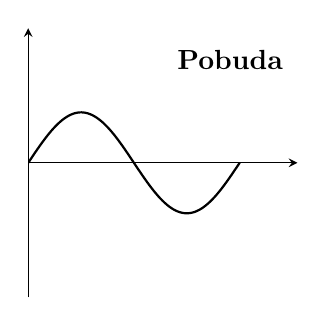
\begin{tikzpicture}
    \begin{axis} [
        title style={at={(0.75,0.75)},anchor=south,yshift=-0.1},
        title = \bfseries{Pobuda},
        ticks = none,
        width = 5cm, height = 5cm,
        xmin = 0, xmax = 8,
        ymin = -2, ymax = 2,
        axis x line = center,
        axis y line = center
    ]
        \addplot [
            domain  = 0:6.283185307179586,
            samples = 100,
            color   = black,
            thick,
        ]{0.75 * sin(deg(x))};
    \end{axis}

\end{tikzpicture}

    \end{subfigure}
    \hskip 1pt
    \begin{subfigure}{0.3\textwidth}
        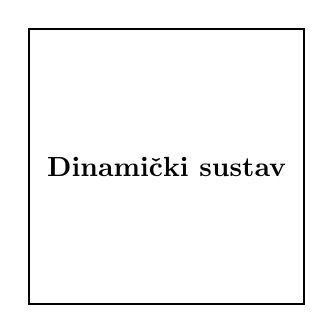
\begin{tikzpicture}
    %sustav
    \draw[thick] (0, 0) rectangle (3.5, 3.5); 
    \node at (1.75, 1.75) {\bfseries{Dinamički sustav}};
\end{tikzpicture}

    \end{subfigure}
    \hskip 1pt
    \begin{subfigure}{0.3\textwidth}
        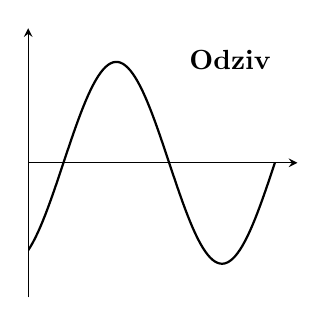
\begin{tikzpicture}
    \begin{axis} [
        title style={at={(0.75,0.75)},anchor=south,yshift=-0.1},
        title = \bfseries{Odziv},
        ticks = none,
        width = 5cm, height = 5cm,
        xmin = 0, xmax = 8,
        ymin = -2, ymax = 2,
        axis x line = center,
        axis y line = center
    ]
        \addplot [
            domain  = 0:7.330382858376184,
            samples = 100,
            color   = black,
            thick,
        ]{1.5* sin(deg(x) - deg(1.047197))};
    \end{axis}

\end{tikzpicture}

    \end{subfigure}
    \caption{Shematski prikaz dinamičkog sustava}
    \label{fig:shematski_prikaz_sustava}
\end{figure}

Sa shematskoga prikaza \ref{fig:shematski_prikaz_sustava} može se naslutiti da su pobuda 
i odziv u međusobnoj sprezi. Navedenom spregom "upravlja" dinamički sustav. U slučaju da 
dinamički sustav pripada razredu linearnih sustava, sprega između pobude i odziva zadana 
je konvolucijom pobude s prijenosnom funkcije sustava. Sama prijenosna funkcija određena 
je diferencijalnom jednadžbom sustava. 
\par

%Većina dinamičkih sustava iz tehnologije zaista spada u kategoriju linearnih sustava. 
%Da bi određeni dinamički sustav bio i linearni sustav mora zadovoljiti slijedeća 
%svojstva: 
%\begin{enumerate}
%    \item aditivnost
%    \item homogenost
%    \item fazni pomak u pobudi rezultira identičnim faznim pomakom u odzivu
%    \item statička linearnost - nije nužan uvjet, ali je poslijedica prethodna tri
%\end{enumerate}
%
%\par
%Objasni svojstva
%\par

U ovome se radu razmatra mehanički linearni sustav najprije s jednim, a
zatim i s više stupnjeva slobode pod utjecajem harmonijske sile $p(t) = p_0 \sin(\omega t)$. 
Teorijski koncepti izvedeni za linearni sustav s jednim stupnjem slobode koriste se  
u razvoju eksperimentalnih metoda za određivanje perioda stupnja prigušenja realnih 
konstrukcija. 
\par

Cilj ovog rada jest upoznavanje s osnovnim teorijskim i praktičnim znanjima iz
dinamike konstrukcija. 

